
\section{Von Neumann Probability}

\label{subsec:int_von_neumann_probability}

%In the introdutory section regarding Quantum Computation we could note that probabilities are an intrinsic part of quantum theory.

 
In the beginning on the $20^{th}$ century the nature of light was once again in the spotlight. The question whether light would be a particle (corpuscular theory), or a wave (undulatory theory), was posed throughout History. Newton, notoriously, considered light to be a particle and presented arguments such as the fact that light travels in a straight like, not bending when presented with obstacles, unlike waves, and gave an interpretation of the diffraction mechanism by resorting to a special medium (aether), where the light corpuscles could create a localized wave\cite{DiasdeDeus:1387968}. 

%figura difracção

The idea of light as a particle stood up until the $18^{th}$century as many scientists (Robert Hooke, Christian Huygens and Leonhard Euler to name a few) tried to explain contradictions found in corpuscular theory. This brought back the idea that light behaves like a wave. 

One of the most famous experiments that corroborates the undulatory theory is the Young's experiments ($19^{th}$ century), or the double-slit interferometer.

%figura double-slit
\begin{figure}[h]
\centering 

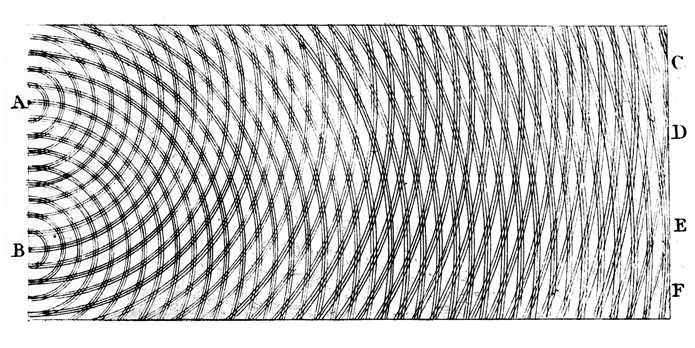
\includegraphics[scale=0.25]{Overview/Figures/Young_Diffraction.png}

\caption[Caption for LOF]{Thomas Young's sketch of two-slit diffraction of light. \footnote}

\label{fig:double_slit}
\end{figure}
\footnotetext{Source: Young, Thomas: Probability. \url{http://en.wikipedia.org/wiki/File:Young_Diffraction.png (1803)}}

The apparatus for the double-slit experiment can be seen in Figure \ref{fig:double_slit}. A light source is placed in such a way that ``two portions" of light arrive at same time at the slits. Behind the barrier is a ``wall" placed to intercept the light. 
The light captured at a wall will sport an interference pattern similar to the pattern when two  waves interfere.
The double-slit experiment was considered for a while the full stop on the discussion on the nature of light.
However with experiments on the spectres of the light emitted by diverse substances and its relation with temperature, a new problem was posed. 

%figura black-body

The black body radiation problem was the theoretical problem where a body that absorbs light in all the electromagnetic spectrum, this makes the body acting as an natural vibrator, where each mode would have the same energy, according to the classic theory. 

When a black body is at a determined temperature the frequency of the radiation it emits depends on the temperature. The classic theory predicted that most of the energy of the body would be in the high frequency part of the spectrum (violet part) where most modes would be found, this led to a prediction called the ultraviolet catastrophe. According to the classic theory the black body would emit radiation with an infinite power for temperatures above approximately 5000K. 
Max Plank(1901), provided an explanation where the light was exchanged in discrete amounts called quanta, so that each frequency would only have specific levels of energy. Plank also determined through experimentation the value of the energy of the quanta that became known as photons later, that value became the physical constant called Plank constant:

\begin{equation}
\label{eq:plankconstant}
h = 6.62606957(29) \times 10^{-34} J.s
\end{equation}

In 1905, Einstein used the concept of quanta (photons) to explain the photoelectric effect. 
De Broglie(1924), suggested that that all the matter had a wave-particle duality. This prediction was confirmed by studying the interference patterns caused by electron diffraction.


\subsection{Mathematical Foundations of Quantum Probability} 

As previously explained, Quantum Theory is a branch of physics that has arised from the need to explain certain phenomena that couldn't be explained with the current classical theory.
In the beginning of the 20\textsuperscript{th} century Dirac and von Neumann  helped to create the mathematical formalisms to comprise this theory \cite{sep-qt-nvd}\cite{Summers2006}. 

Von Neumann's contributions were focused in the mathematical rigor, as is framework is strongly based in Hilbert's theory of operators. Dirac's concerns were more of a practical nature. Their combined contributions were invaluable to establish the this area. 

From Dirac it's important to point the Dirac's notation (also known as Bra-ket notation or  $\langle Bra\vert c\vert ket\rangle$ ) (introduced in 1939 \cite{sep-qt-nvd}), that is widely used in literature based on quantum theory. This notation uses angle brackets and vertical bars to represent quantum states (or abstract vectors) as it can be seen in the formulas \eqref{langle_dirac} and \eqref{rangle_dirac}. 

\begin{equation}
\label{langle_dirac}
\langle z\vert=\left[\begin{array}{cccc}
z_{1} & z_{2} & ... & z_{n}\end{array}\right]
\end{equation}

\begin{equation}
\label{rangle_dirac}
\vert z\rangle = ( \langle z\vert )^*  =\left[\begin{array}{c}
z_{1}\\
z_{2}\\
...\\
z_{n}
\end{array}\right]
\end{equation}


%of two quantum states ($\langle \phi \vert \psi \rangle$)
This notation provides for an elegant representation of the inner product \eqref{eq_inner} and verifies the has linearity as it follows in equation \eqref{eq_linearity}. While the Bra-ket notation can be useful in terms of condensing information, using vectors and matrixes to represent the states turns out to be a more approachable way to understand and manipulate data.
 

\begin{equation}
\label{eq_inner}
\langle z\vert z\rangle={\displaystyle \sum_{i=1}^{n}\bar{z_{i}}z_{i}}
\end{equation}
where $\bar{z_{i}}$ is the complex conjugate of $z_{i}$.

 

\begin{equation}
\label{eq_linearity}
\langle z\vert(\alpha\vert x\rangle+\beta\vert y\rangle)=\alpha\langle z\vert x\rangle+\beta\langle z\vert y\rangle
\end{equation}


\subsubsection{Born rule}

The Born rule was formulated by Born in 1926. This law allows to predict the probability that a measurement on a quantum system will yield a certain result. This law provides a link between the mathematical foundation of Quantum Mechanics and the experimental evidence\cite{VanRijsbergen2004}\cite{Landsman2009}. 

A quantum system is represented by a n-dimensional Hilbert Space, a complex vector space in which the inner product is defined. In the Figure \ref{fig:circle} we have a representation of quantum state $\vert v \rangle$ in a two-dimensional Hilbert Space. 

\begin{figure}[h]
\centering 

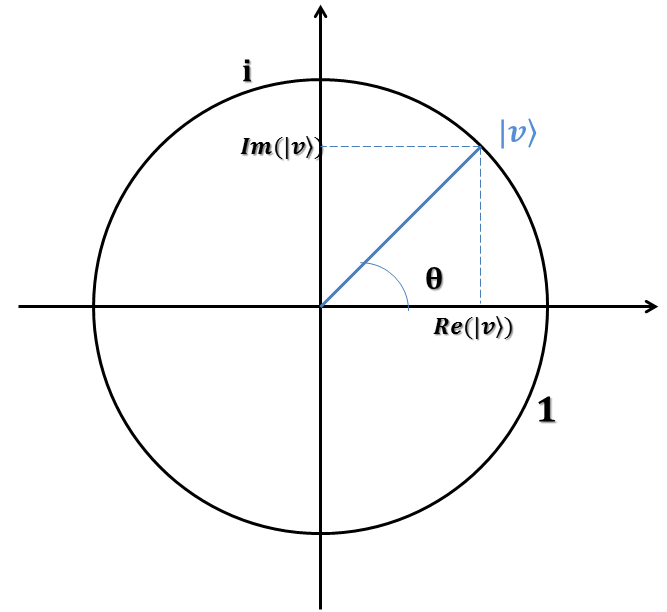
\includegraphics[scale=0.35]{Overview/Figures/complex_circle.png}
\caption{Representation of a two-dimensional Hilbert Space($H^{2}$)}
\label{fig:circle}
\end{figure}

The Born rule states that if there is a system is in a state $\vert v \rangle$  (in a given n-dimensional Hilbert Space $H$ ), and an Hermitian operator $A$ is applied then the probability of measuring a specific eigenvalue $\lambda_{i}$ associated with the i-th eigenvector of $A$ ($\psi_{i}$), will be given by\cite{VanRijsbergen2004}: 


\begin{equation}
\label{eq_born_rule}
P_{v}(\lambda_{i}) = \langle v\vert Proj_{i}\vert v\rangle
\end{equation}

where $Proj_{i}$ is a projection matrix corresponding to $\psi_{i}$ :

 \begin{equation}
\label{eq_born_rule_1}
Proj_{i} = \vert\psi_{i}\rangle \langle \psi_{i}\vert
\end{equation}

Given the properties of A, the set of eigenvectors $\{ \psi_{1}, \psi_{2}, ..., \psi_{i},..., \psi_{n}\}$ forms a orthogonal basis of the n-dimensional Hilbert Space considered. Thus the state $\vert v \rangle$
can be written as a linear combination of the eigenvectors of A:

 \begin{equation}
\label{eq_born_rule_lala}
\vert v \rangle = \alpha_{1}\psi_{1}+ \alpha_{2}\psi_{2}+ ...+\alpha_{i}\psi_{i}+...+\alpha_{n}\psi_{n}
\end{equation}

The coefitients $\alpha_{i}$ are complex numbers called probability amplitudes, and their squared sum is equal to 1: 
\begin{equation}
\sum_{i=0}^{n} \vert \alpha_{i}\vert^{2} = 1
\end{equation}

this brings us to: 

\begin{equation}
\label{eq_born_rule_2}
P_{v}(\lambda_{i}) =\langle v\vert\psi_{i}\rangle\langle\psi_{i}\vert v\rangle=\vert\langle v\vert\psi_{i}\rangle \vert^{2} = \vert \alpha_{i}^{*}\alpha_{i}\vert^{2}
\end{equation}

So the determination of the probability of an event ($P(A)$ ),
is made by projecting the quantum state in the basis $A$ of the
Hilbert Space and measuring the squared length of the projection.\cite{Trueblood}

$P(A)=\left(Proj_{A}\vert z\rangle\right)^{2}$ 

Applying an operator can be seen as applying a rotation matrix on the system ($\vert v \rangle$) and measuring the projection of $\vert v \rangle$ onto the imaginary axis and the real axis (Figure \ref{fig:circle}), or considering that we have a determined state vector and rotating the orthogonal basis of the Hilbert Space according to an operator and then to do a projection on the new chosen orthogonal basis.

According to Leiffer\cite{Leifer2008} ``quantum theory can be thought of as a non-commutative, operator-valued, generalization of classical probability theory". 

%traces and density operators

As in the classical probability theory where from a random variable it is possible to establish a probability distribution, also known as density function, in the Hilbert space there is a equivalent density operator.
The density operator ($\rho$) is a Hermitian operator that has the particularity of having its trace equal to 1\cite{VanRijsbergen2004}.

\begin{equation}
\label{eq_trace1}
\rho = \sum_{i=0}^{n} \alpha_{i} \vert\psi_{i}\rangle\langle\psi_{i}\vert
\end{equation} 

\begin{equation}
\label{eq_trace1}
tr( \rho ) = 1
\end{equation}

\subsubsection{Example of the double-slit experiment with electrons}
 Like the Young's Experiment with light created an interference pattern similar to a wave, firing electrons one at the time produces a similar pattern. The unobserved fired electron behaved like a wave and after passing the slits the wavelets interfered with one another to create a interference pattern. However if a measuring device was active while the electron was fired the interference pattern wasn't registered. 

\begin{figure}[h]
\centering 
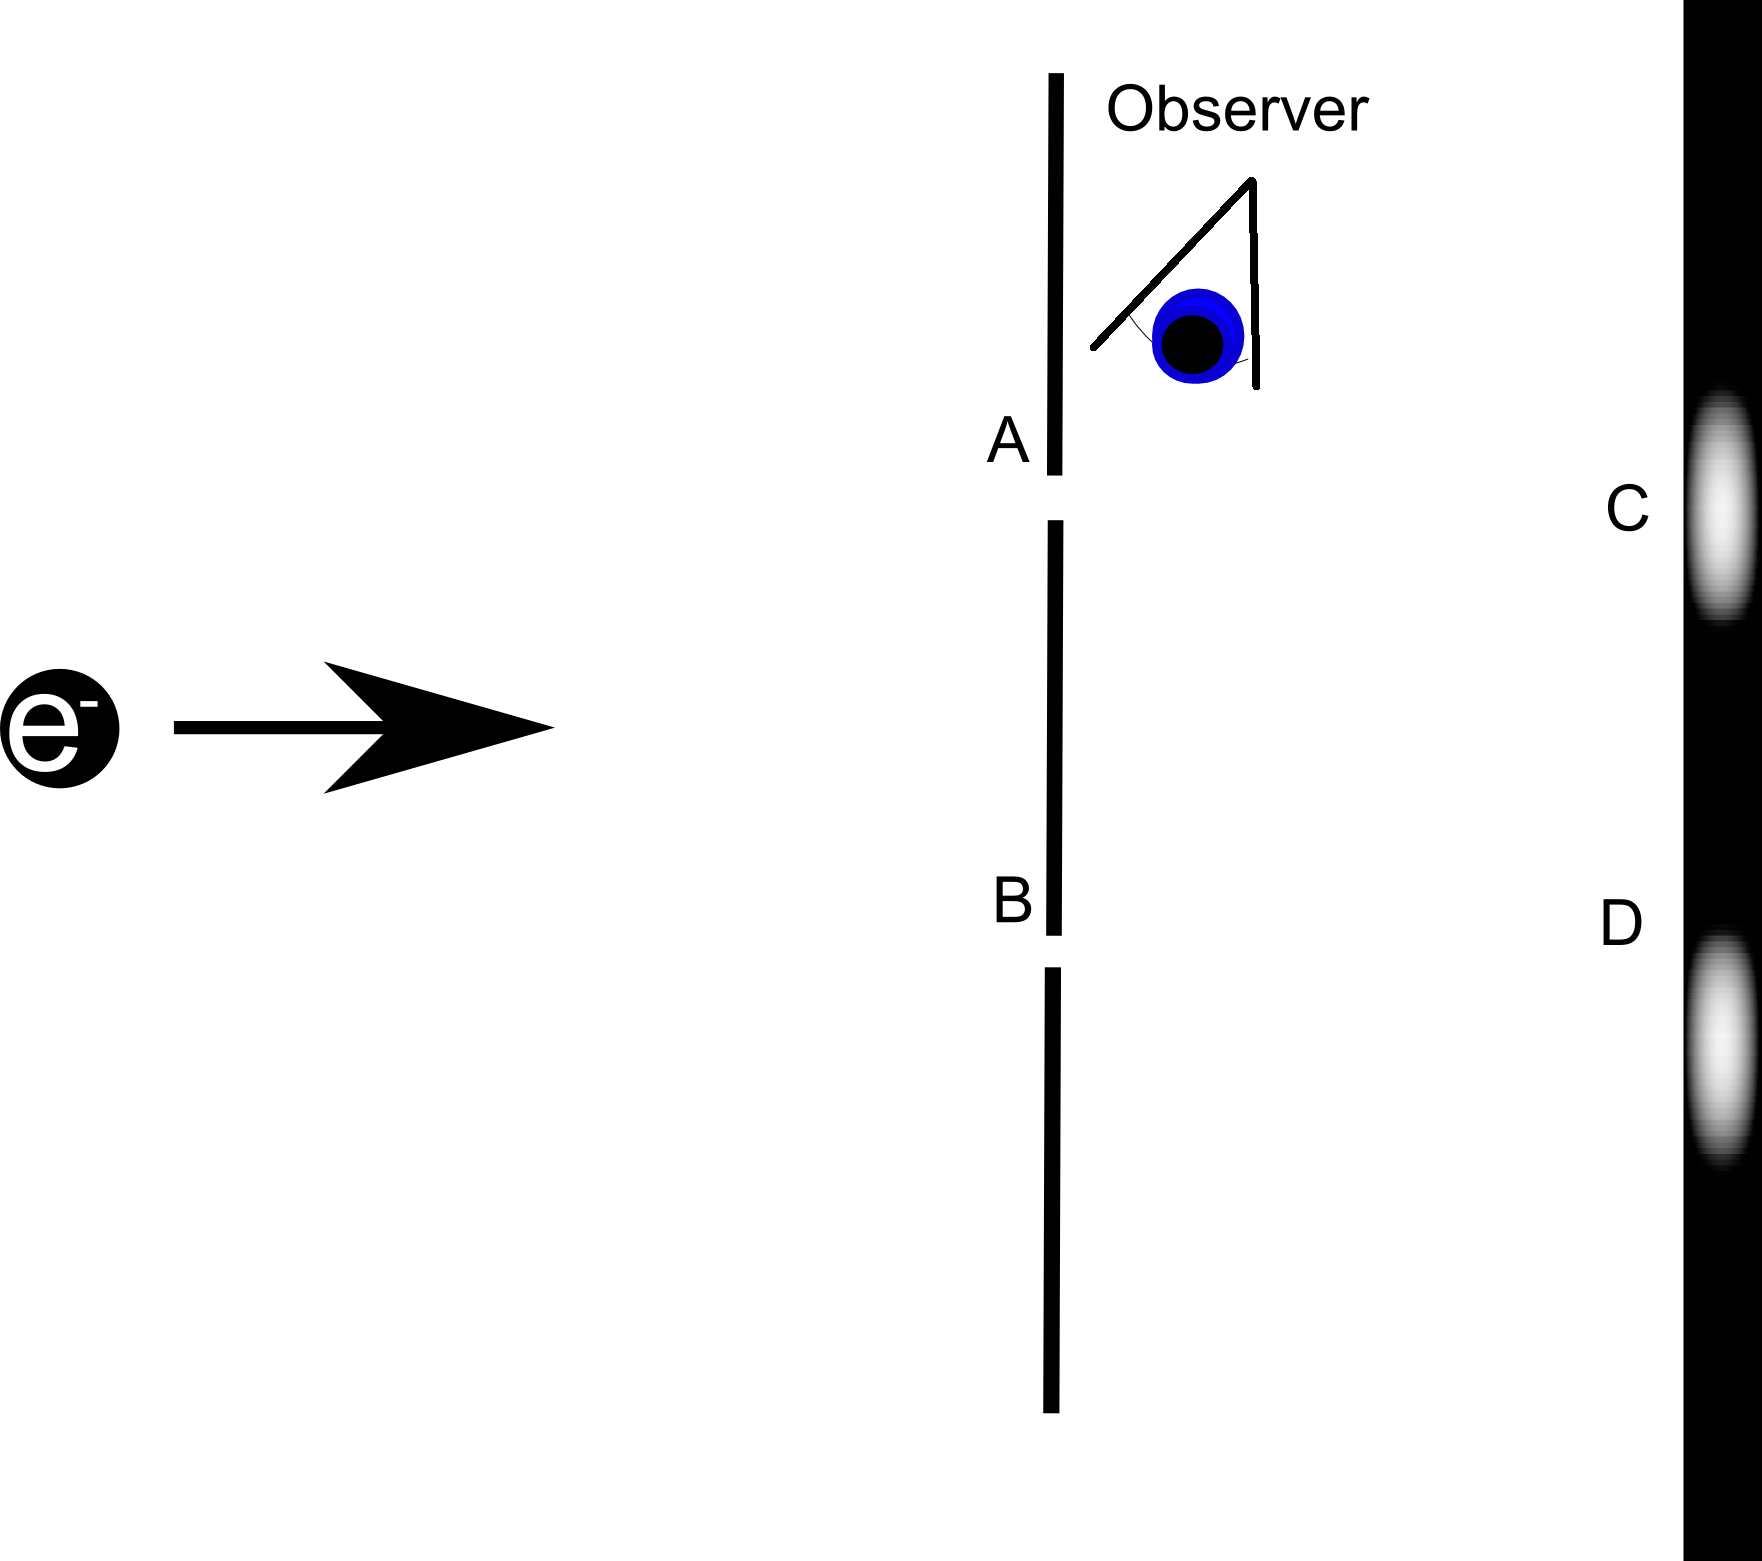
\includegraphics[scale=0.15]{Overview/Figures/ds_ob.png}
\caption{Double-slit experiment where there's a measuring device that allows to know through which slit the electron passed.}
\label{fig:double_slit_ob}

\end{figure}
\begin{figure}[h]
\centering 

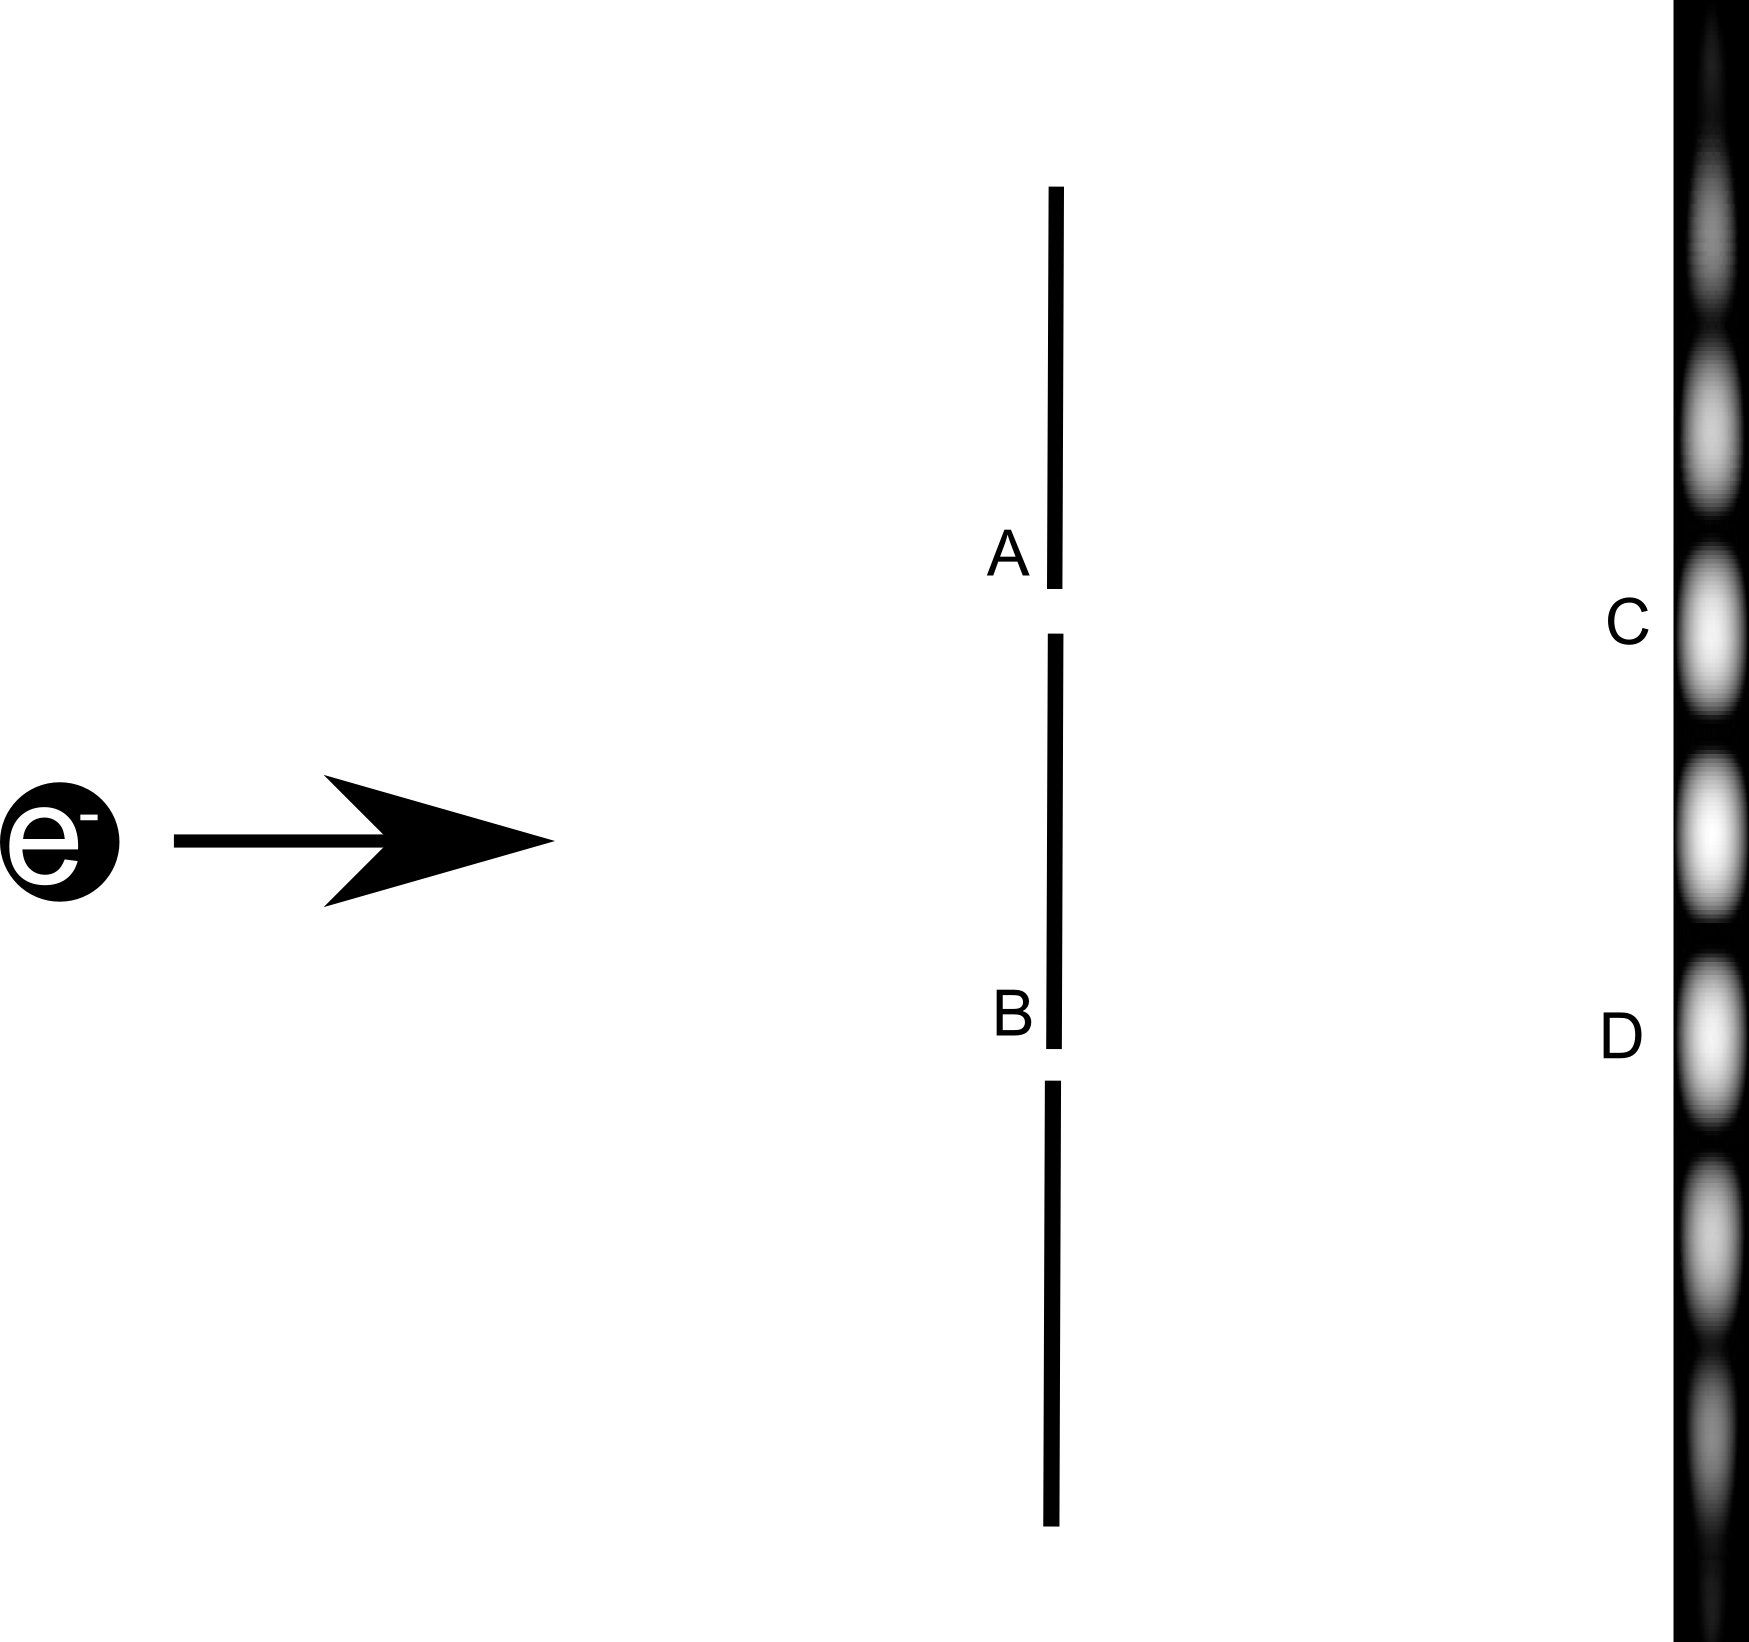
\includegraphics[scale=0.15]{Overview/Figures/ds_unob.png}
\caption{Double-slit experiment, where the electrons exibit the interference pattern characteristic in waves}
\label{fig:double_slit_unob}
\end{figure}

The fact that the electron was measured while passing through a slit produced a particle behaviour, explained by the classical theory (Figure \ref{fig:double_slit_ob}). 


In this experiment a single electron is shoot at a time. So in the start of the experiment (S), we know the initial position of the electron, this corresponds to the.

A final measurement (F) is made when the electron hits the wall behind the slits, where we know the final position of the electron.
\footnote{Mohrhoff, U.: Two Slits. \url{ http://thisquantumworld.com/wp/the-mystique-of-quantum-mechanics/two-slit-experiment/#fn1back}}

If this experiment is observed, there is an intermediate measure that tells us whether the electron went throught the slit A or B. The corresponding probability amplitudes related to this measurement are $\omega_{A}$ and $\omega_{B}$, and:
\begin{equation}
\omega_{A} = \langle F \vert A\rangle \langle A \vert S\rangle
\end{equation}
\begin{equation}
\omega_{B} = \langle F \vert B\rangle \langle B \vert S\rangle
\end{equation}

If we consider the intermediate measurement the probability $P(F\vert S)$ will be:
\begin{equation}
P(F\vert S) = 
\vert \langle F \vert A\rangle \langle A \vert S\rangle \vert^{2}
+
\vert \langle F \vert B\rangle \langle B \vert S\rangle \vert^{2}
\end{equation}

But if we only measure the position of the electron at the end of the experiment that probability will be:
\begin{equation}
P(F\vert S) = 
\vert \langle F \vert A\rangle \langle A \vert S\rangle 
+
 \langle F \vert B\rangle \langle B \vert S\rangle \vert^{2}
\end{equation}
The latter equation will be dependent on a interference coefficient that will be responsible the interference pattern observed in the unobserved experiment.

\begin{comment}
According to the Uncertainty principle, by Heisenberg, the precision with which we can know the position and momentum of a particle-wave is constrained, and higher certainty relative to the position bring higher uncertainty in terms of its velocity. When we observe the electron we gain certainty relative to its position, but at the same time we are conditioning its momentum. In the unobserved experiment the interference pattern allows us to calculate the characteristics of the wave but at the same time there's a greater uncertainty associated with the position of the electron there are more strips where it is highly probable to find the electron.
\end{comment}


\subsubsection{Example of the Polarization of Light}
The photons in a beam of light don't vibrate all the same direction in most of the natural sources of light. To filter the light polaroids are used. A polaroid only allows the passage of light in a well-defined direction and thus reducing the intesity of the light. In the Figure \ref{fig:polaroids} we can observe that the introduction of the oblique polaroid in the third situation led to a passage of light. Although there is a classical explanation to this phenomenon if we consider waves when we are considering a beam of light, if our light source emits one photon at the time a quantum mechanical explanation is needed\cite{Rieffel2011}.

\begin{figure}[h]
\centering 

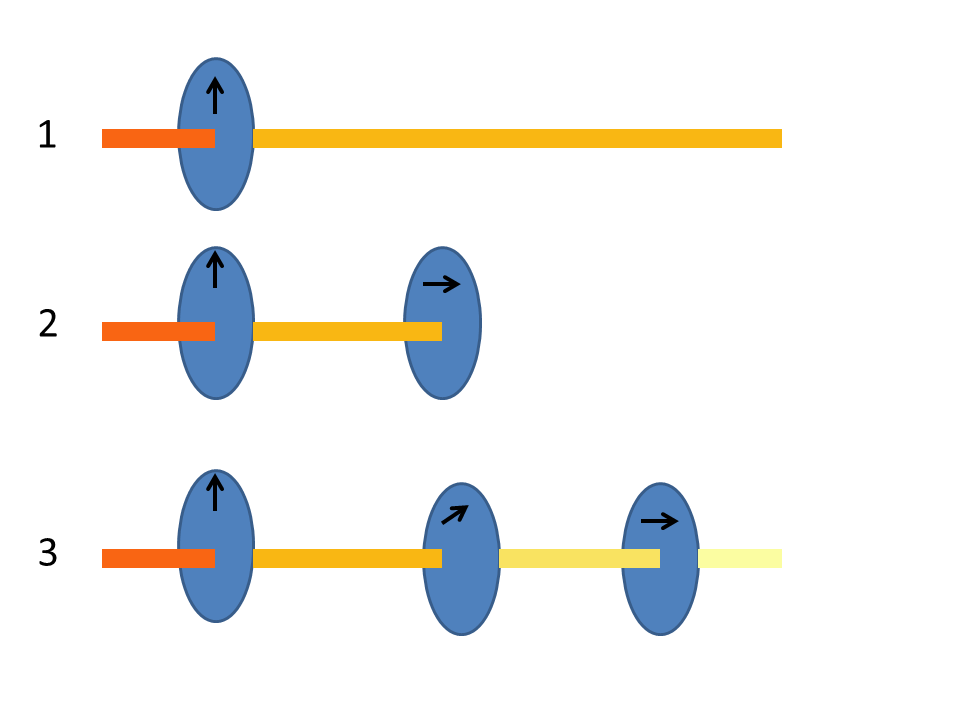
\includegraphics[scale=0.25]{Overview/Figures/Polaroids.png}
\caption{1. With one vertical polaroid the unpolarized light is attenuated by a half. 2. Vertical polarization followed by a horizontal polarization will block all the passing light. 3. Inserting a oblique polaroid between the vertical and horizontal polaroids will allow light to pass.}
\label{fig:polaroids}
\end{figure}

To model the photon's polarization in a quantum setting, we will use a vector $\vert v \rangle $ in a two-dimensional Hilbert Space: 
\begin{equation}
\vert v \rangle = a\left[\begin{array}{c}
1\\
0
\end{array}\right]+ b\left[\begin{array}{c}
0\\
1
\end{array}\right]
\end{equation}

where $\left[\begin{array}{c}
1\\
0
\end{array}\right]$ would represent the vertical direction (could also be represented by the state vector $\vert\uparrow\rangle$), and $\left[\begin{array}{c}
0\\
1
\end{array}\right] $ the horizontal one (another possible representation to this basis could be $\vert\rightarrow\rangle$). We can consider the Figure \ref{fig:circle} as a graphical representation for this system.

In the first situation if $a = \frac{1}{\sqrt{2}}$, that would mean that the probability of passing the vertical polaroid would be $a = (\frac{1}{\sqrt{2}})^{2} = 0.5$, that would light to the expected reduction of a half of the intensity of light. After passing throught the vertical polaroid the photon will have a polarization of $\vert v \rangle = a\left[\begin{array}{c}
1\\
0
\end{array}\right]$. Considering now the second situation after we have our photon polarized vertically (like in the end on the first situation), the probability of being vertically polarized is 1, thus making the probability of passing throught the horizontal polaroid 0.
In the third situation, after being vertically polarized the photon will pass throught an oblique polaroid that makes its direction

\begin{equation}
\vert v \rangle = i.sen(\theta) \left[\begin{array}{c}
1\\
0
\end{array}\right]+ cos(\theta)\left[\begin{array}{c}
0\\
1
\end{array}\right]
\end{equation}



$\theta$ being the angle of the polaroid. The photon filtered by the vertical polaroid will pass this second polaroid with a probability of $(i.sen(\theta))^{2}$, becoming polarized according to the filter, as we can observe depending on the value of $\theta$ we will now have a horizontal component in the vector that describes the state of the photon. This will make the photon pass the horizontal polaroid  with a probability of $cos(\theta)^{2}$. 
%\nearrow


\subsection{Quantum Computing}
\label{subsec:int_quantum_computing}


%\subsection{Introduction}
%\label{subsec:int_int_quantum_computing}



The quantum equivalent of a bit (the basic unit of information in computers), is a qubit (or quantum bit). A qubit is a two-state quantum system that can be interpreted as a normalized vector in a two-dimensional Hilbert space. This Hilbert ($H^2$), space has two basis (also known as pure states). In quantum computing, the basis used are ${ \vert 0 \rangle , \vert 1 \rangle }$ or $\left[\begin{array}{c}
1\\
0
\end{array}\right]$
 and 
$\left[\begin{array}{c}
0\\
1
\end{array}\right]$ 

The qubit can be described in terms of linear transformations of pure states as in \eqref{qubit}, $\omega_{0}$ and $\omega_{1}$ are complex numbers called probability amplitudes. When a system is in a mixture of this pure states (as the general representation in \eqref{qubit} might point), it is in a phenomenon known as superposition. Measuring forces the system to collapse and assume one of the pure states with a certain probability. 

\begin{equation}
\label{qubit}
\vert \psi \rangle = \omega_{0}\vert0\rangle+\omega_{1}\vert1\rangle = \left[\begin{array}{c}
\omega_{0}\\
\omega_{1}
\end{array}\right]
\end{equation}

In the example stated in the representation \eqref{qubit} the probability of the system falling into the state $\vert 0 \rangle $ would be $\vert\omega_{0}\vert^{2}$ . The probability of the system falling into $\vert 1 \rangle $ would be $\vert\omega_{1}\vert^{2}$ . The second axiom of Kolmogorov (law of total probability) is verified (\eqref{2nd_axyom}).

\begin{equation}
\label{2nd_axyom}
\vert\omega_{0}\vert^{2}+\vert\omega_{1}\vert^{2}=1
\end{equation}

%So considering again the inner product  ($\langle \phi \vert \psi \rangle$) we can verify that it holds a physical interpretation: the probability amplitude of the state %$\psi$ collapsing into $\phi$ .
 
$\omega_{0}$ and $\omega_{1}$ (\eqref{qubit}) are complex numbers, the so-called probability amplitudes. When squared, the probability amplitude represents a probability. 

\begin{comment}
We can define linear operators in the Hilbert space, one of the most important classes of operators being the self-adjoint operators,  $A = A^{*}$, that have the property stated in \eqref{eq_adjoint}. The Hermitian operator is one that satisfies the property of being equal to its conjugate transposed, $A = A^{*T} =A^\dagger$ .  In a finite-dimensional Hilbert space defined by a set of orthonormal basis every self-adjoint operator is Hermitian.

\begin{equation}
\label{eq_adjoint}
\langle A^{*}z\vert x\rangle=\langle z\vert Ax\rangle
\end{equation}

Observables are deemed as the physical properties that can be measured. One way to think of them is to consider the 20 question game, where a two player game where one person thinks of an object and then the second person has a set of 20 "Yes" or "No" to discover the object, one observable could be "Is it red?". With each question the space comprising the possible answers will not increase, this means that asking two times in a row if the object is red in the game will always yield the same answer.
 
Hermitian operators are suitable for being used as observables, as their eigenvalues are real numbers.
The eigenvectors associated with the eigenvalues of the observable will correspond to the state in which the system will be after applying the Hermitian operator. Thus applying an observable to the system can be viewed as doing a projection of the system in the basis formed by the eigenvectors.  
\end{comment}

\subsubsection{Compound Systems}

The representation of a system comprising multiple qubits grows exponentialy. If to represent a single qubit system there is a two-dimensional Hilbert space, to represent a system with m qubits a $2^m$-dimension space would be required. This growth when we have a multiple-qubit system is achieved by a tensor product among the single systems that are a part of it.

%Tensor product
The tensor product is an operation denoted by the symbol $\otimes$. 
Given two vector spaces V and W with basis 
\begin{equation}
A = \left\{ \vert \alpha_{1} \rangle, \vert \alpha_{2} \rangle , ..., \vert \alpha_{m} \rangle \right\}\end{equation} and 
\begin{equation} B = \left\{ \vert \beta_{1} \rangle, \vert \beta_{2} \rangle , ..., \vert \beta_{n} \rangle \right\}\end{equation} respectively, their tensor product would be the mn-dimensional vector space with a basis with elements of the form $ \vert \alpha_{i} \rangle \otimes \vert \beta_{j} \rangle$\cite{Rieffel2011}.

For example, if we consider two Hilbert spaces $H^2$ with basis
$ A=\left\{ \vert 0 \rangle , \vert 1 \rangle \right\}$ and 
$B =\left\{ \vert - \rangle, \vert + \rangle \right\}$
, their tensor product would be a $H^4$ with basis:
\begin{equation}
AB = \left\{ \vert 0  - \rangle, \vert 0 + \rangle, \vert 1 - \rangle,  \vert 1 + \rangle \right\}
\end{equation}

The Bra-ket notation provides a way to prevent the escalation of the basis notation. When specified the vector space the basis can be specified in base 10 for simplicity sake. According to this the basis of the last example would be $AB = \left\{ \vert 0 \rangle, \vert 1 \rangle, \vert 2 \rangle,  \vert 3 \rangle \right\}$.

\subsubsection{Entanglement}
In multiple qubit systems, qubits can interfere with each other, thus making impossible to determine the state of part of the system without ``disturbing" the whole. In other words, there are states in a multi-qubit system that can't be described as a tensor product of single-qubit systems; this superposition is called quantum entanglement. This property is not local as transformations that act separately in different parts of an entangled system can't break the entanglement. Quantum entanglement is one of the core aspects when we're trying to explore the full potential of quantum systems \cite{Rieffel2011}.

For example let's consider following quantum states, known as Bell states:
\begin{equation}
\vert\Phi^{+}\rangle=\frac{1}{\sqrt{2}}(\vert0\rangle_{A} \otimes\vert0\rangle_{B} +\vert1\rangle_{A} \otimes\vert1\rangle_{B})=\frac{1}{\sqrt{2}}(\vert00\rangle+\vert11\rangle)
\end{equation}
\begin{equation}
\vert\Phi^{-}\rangle=\frac{1}{\sqrt{2}}(\vert0\rangle_{A} \otimes\vert0\rangle_{B} -\vert1\rangle_{A} \otimes\vert1\rangle_{B})=\frac{1}{\sqrt{2}}(\vert00\rangle-\vert11\rangle)
\end{equation}


\begin{equation}
\vert\Psi^{+}\rangle=\frac{1}{\sqrt{2}}(\vert0\rangle_{A} \otimes\vert1\rangle_{B} +\vert1\rangle_{A}\otimes\vert0\rangle_{B})=\frac{1}{\sqrt{2}}(\vert01\rangle+\vert10\rangle)
\end{equation}


\begin{equation}
\vert\Psi^{-}\rangle=\frac{1}{\sqrt{2}}(\vert0\rangle_{A} \otimes\vert1\rangle_{B} -\vert1\rangle_{A} \otimes\vert0\rangle_{B})=\frac{1}{\sqrt{2}}(\vert01\rangle-\vert10\rangle)
\end{equation}

These states are a particular basis in $H^2$ as they are all entangled states and they are maximally entangled. Let's suppose that we have a system of two qubits in a Hilbert space in the mixed state $\vert\Phi^{+}\rangle$ if we measure the qubit A (by deciding the outcome $0$ or $1$ with a probability of $0.5$ for each),we are automatically uncovering the value of the qubit B. In this state we know the second qubit will always yield the same value of the first measured qubit. Se second value is correlated with the first one.



\begin{comment}
	\item Born Rule probabilities
falar aqui das funções oraculo
\end{comment}

%%%%%%%
%% Probabilities

%%%%%%%
%% QBN

%
\subsection{Quantum Bayesian Networks}

\label{subsec:int_QBN}

The use of graphs and visual depictions devised to work with quantum mechanics allows for an abstraction from the mathematical formulas behind the systems. This is the idea behind the Feynman Diagrams, that have been used extensively as David Kaiser confirms\cite{Kaiser2005}. Using a \ac{QBN} could provide an interesting way to represent data, namely conditional dependencies, and therefore be a valuable tool when dealing with quantum probabilities in large systems.  

A proposition for a \ac{QBN} model was first mentioned by Tucci\cite[1997]{Tucci1997}. The motivation behind \acs{QBN} would be the construction of a framework to calculate quantum mechanical conditional probabilities, and the followed approach was to alter the minimum possible its classic counterpart so that it would allow for working with quantum mechanics.

The main idea featured in this first approach\cite{Tucci1997} dealt with quantum pure states. According Tucci, ``a QB net for a pure state consists of a directed acyclic graph (DAG) and a transition matrix (a complex matrix), assigned to each node of the graph" \cite{Tucci2012} and that ``keeping QB nets[Quantum Bayesian Networks] close to CB nets[Bayesian Networks] can be very fruitful, because much is already known about CB nets"\cite{Tucci2012}. It's also enforced that each node has a numerical value and the whole graph also possesses a numerical value (the product of nodes), so factorization should be similar to their classical version.
The \ac{QBN} would be \ac{DAG} labelled with a collection of node matrices. Each node has a random variable attached to it and a matrix containing probability amplitudes (complex numbers). 
In its introductory article regarding Quantum Bayesian Networks, Tucci writes that ``keeping QB nets close to CB nets can be very fruitful, because much is already known about CB nets"\cite{Tucci2012}. Tucci also points an example of usage of \ac{QBN} in medical diagnosis\cite{Tucci2008}.


Meanwhile other approaches were formulated namely Leifer's\cite{Leifer2008} in his article "Quantum Graphical Models for Belief Propagation", that focus on attributing a density matrix to each node. This would be the equivalent of attributing a known probability function (like a Gaussian distribution), to each variable. 



% Examples!!!!




 




\subsection{Quantum Cognition}
\label{subsec:QuantumCog}

The idea of resorting to quantum mechanics to explain phenomena underlying consciousness has been pointed in literature by the founding fathers of quantum mechanics, and starts to acquire importance in the neuroscience community, that seeks and recognizes that the analysis of dendrite-synapse fall into the spatio-temporal level explained by quantum mechanics\cite{Tarlaci2010}. 

Quantum Cognition is an area that applies the formalism of quantum theory to model to interpret cognitive phenomena. 
Some of the reasons pointed by Trueblood and Busemeyer\cite{Trueblood}\cite{Busemeyer:2012:QMC:2385442} to adopt a quantum approach to cognitive science are:
\begin{itemize}
\item The inference process is considered a construction; 
\item Ambiguity can be felt;
\item Interference between beliefs and uncertainty are possible. 
\end{itemize}

There is empirical evidence that our beliefs could be more accurately explained by a quantum model than a classical model, as there are numerous paradoxes that arise when we apply classical probability frameworks to describe human inference process\cite[Busemeyer et al]{Busemeyer2009}. 
Paradoxes such as the ``Allais paradox" and the ``Ellsberg paradox", point for inconsistencies between the expected utility hypotesis and experimental results\cite{Aerts2011}.

For example, the commutative property of events relating to the disjunction, does not accommodate the fact that it is verified\cite{TruebloodJ} that in human inference process, order affects the probability of a hypothesis given a sequence. The order of questions in a quiz is an example on disjunction where this is verified. By altering the order of the questions  in a questionnaire the results will be vary. \cite{Trueblood}

\subsubsection{Example of a Conjunction and Disjunction Fallacy}
To illustrate a disjunction fallacy \cite[Busemeyer et al]{Busemeyer2009} a short story was presented to subjects and then it was asked of them to emit an opinion about the likelihood of a two prepositions based on the story.
The story is about ``a liberal philosophy student from Berkeley named Linda.'' and the hypothesis presented deal with her future occupations:
\begin{enumerate}
\item Linda will be a bank teller;
\item Linda will be a bank teller and a feminist.
\end{enumerate} 

People identify the likelyhood of Linda being a feminist high (H). The fact that she's now a bank teller doesn't seem very plausible, thus being considered low (L). Nonetheless, despite the law of probability stating that the hypothesis 1 will have a higher probability than hypothesis 2 ($P(Bank Teller) \geq P(Bank Teller \wedge Feminist)$), people systematically think it's the other way around (85\% of 142 participants), rendering us with a conjunction fallacy, where judgement:
\begin{equation}
J(L) \leq J(L \wedge H)
\end{equation}

When considering the hypothesis:
\begin{enumerate}
\item Linda will be a feminist;
\item Linda will be a bank teller or a feminist.
\end{enumerate}
A disjunction fallacy was found as:
\begin{equation}
J(H) \geq J(L \vee H)
\end{equation}




\subsubsection{Example on the quantum modelling of the Ellsberg Paradox}

The Ellsberg paradox points outs inconsistencies in the predictions of 
expected utility theory and the human's response, when ambiguity is present. 
People tend to prefer situations with known risks (when we are able to estimate a prior probability), over unknown risks (when we have no information). For 
that matter the notion of ambiguity became more attached with an uncertainty 
that doesn't have a known probability distribution to model it, an unknown 
risk.

In the original formulation of the problem, by Daniel Ellsberg \cite
{Ellsberg} there is a urn containing 30 red balls and 60 balls that can be 
black or yellow. The exact number of black balls is unknown, but the sum of 
black and yellow balls always adds up to 60. Each ball in the urn has equal 
chance of being drawn and two gamble options are presented:

\begin{itemize}
\item A: If a red ball is drawn, there's a payoff of 100\$;
\item B: If a black ball is drawn, there's a payoff of 100\$; 
\end{itemize}

Another gamble is provided with the same urn, in the same conditions:

\begin{itemize}
\item C: If a red ball or a yellow ball is drawn, there's a payoff of 100\$;
\item D: If a black ball or a yellow ball is drawn, there's a payoff of 
100\$; 
\end{itemize}

According to the utility theory the bet A is preferred over the bet B if the 
subject believes that the probability of drawing a red ball is greater than 
the probability of drawing a black ball. according the same principle the bet 
C would be chosen over D. However when testing with subjects, although the 
bet A was chosen over B, the bet D was systematically preferred over C. 

This paradox violates the Sure Thing Principle (or the strong independence assumption), \cite{Savage1954}. Under this assumption the outcome of drawing a red ball and outcome of drawing a black ball are indifferent in themselves, then if we consider the outcome of drawing a red ball or a yellow ball, that probability  must be indifferent to a probability of drawing a black ball or a yellow ball.

The purpose of this paradox is to point out that the worst case scenario is 
taken into account even when there's no information to sustain that option 
over more favourable outcomes. 

To analyse this problem in the domain of 
quantum cognition\cite[Aerts et al]{Aerts2011}, made this experiment with 59 
subjects and tried to model the problem in a quantum way by analysing the 
explanations given by some of the subjects in their reasoning process. They 
identified that the subjects didn't relied only in the physical situation to 
decide which bets to take and identified ``conceptual 
landscapes" that the 
subject had resorted to. They identified 6 of this landscapes.

\begin{itemize}
\item ``Physical Landscape" - a neutral look at the problem directly derived 
from the definition of the problem;
\item ``First Choice Optimistic Landscape" - focus on the belief that there 
might be more black balls than yellow balls relative to the first gamble, 
this leads to a preference for the bet B over A;
\item ``Second Choice Optimistic Landscape" - when presented with the gambles 
C and D, the belief that there are more yellow balls than black balls, 
leading to a preference of C over D.
\item ``First Choice Pessimistic Landscape" - focus on the belief that there 
might be more yellow balls than black relative to the first gamble, leading 
to a preference of A over B;
\item ``Second Choice Pessimistic Landscape" - in the second choice, the 
belief that there are fewer yellow balls, which makes the option D 
preferable over C. 
\item ``Suspicion Landscape" - this considers the hypothesis of placement of 
the yellow and black balls to be biased and that there is some trickery 
involved.
\item ``Don't Bother me with Complications Landscape" - if the situation is 
hard to understand choosing the most simple answer.
\end{itemize}

The quantum model takes into account this landscapes to define a vector per 
landscape. The choice between the bets A and B consist of a projector M, and 
the choice between C and D is represented by the operator N. These 
projections affect the weight of each conceptual landscape. The vector that models this 
situation consists in a superposition of all this conceptual landscapes 
normalized considering the weights associated with each vector.

The expected utility hypothesis has a strong mathematical foundation in the utility theory and yet ``It is indeed well known that concepts combine in human minds in such a way that they show deviations from the expectations that could be drawn in classical set and probability theories. Analogously, subjects take decisions which seem to
contradict classical logic and probability theory.'' \cite[Aerts et al]{Aerts2011}. 

\subsubsection{Example of application of Quantum Probabilities in Quantum Cognition}
This example is due to Wang and Liu\cite{Wang2007}\cite{Busemeyer2011}\cite{Busemeyer2009423}. Given a group of pictures (H) depicting human faces, subjects were asked to:
\begin{enumerate}
\item Categorize the picture as ``Good Guy'' (G) or ``Bad Guy''(B);
\item Decide to act Friendly (F) or Aggressive (A).
\end{enumerate} 

At first participants were asked to state their action (F or A), without reporting their categorization of good or bad (G or B). Secondly the exercise was repeated but the subjects were asked their categorization of G or B, before stating F or A. This study was conducted with 26 participants with 51 observations per exercise (reporting G or B or not), for each picture.

The following results were obtained:
\begin{itemize}
\item $P(A\vert H)$ without reporting G or B - $P(A\vert H)=0.69$;

\item $P(A\vert H)$ after reporting G or B:
\begin{itemize}
\item $P(G\vert H) = 0.17$
\item $P(A\vert G) = 0.42$
\item $P(B \vert H) = 0.83$
\item $P(A\vert B) = 0.63$
\end{itemize}
\end{itemize}

By the classical Law of total probability:
\begin{equation}
P(A\vert H) = P(G\vert H).P(A\vert G) + P(B \vert H) . P(A\vert B) = 0.59
\end{equation}

The results are inconsistent, something that classic probability theory can't naturally explain.
Considering a quantum probability approach where $\langle G \vert H\rangle$ is the probability amplitude to consider the face picture (H), a good guy (G). The probability of classifying the face as a good guy is $\vert \langle G \vert H\rangle \vert ^{2}$.
 \begin{equation}
\vert \langle G \vert H\rangle \vert ^{2} + \vert \langle B \vert H\rangle \vert ^{2} = 1
\end{equation}
Using the same reasoning the probability amplitude for deciding to act aggressively (A) given the categorization of the picture as a good guy (G) is $\langle A \vert G\rangle$. Given the two possibilities to act:
 \begin{equation}
\vert \langle A \vert G\rangle \vert ^{2} + \vert \langle F \vert G\rangle \vert ^{2} = 1
\end{equation}

If we consider a direct transition from H to A, like on the first exercise:
 \begin{equation}
\label{eq:quantum_prob_b}
\vert \langle A \vert H\rangle \vert ^{2} = \vert 
 \langle A \vert G\rangle\langle G \vert H\rangle  + \langle A \vert B\rangle\langle B \vert H\rangle \vert^{2}
\end{equation}

By developing the second branch of the Equation \eqref{eq:quantum_prob_b} we are left with:
 \begin{equation}
\label{eq:quantum_prob_b2}
\vert \langle A \vert H\rangle \vert ^{2} = \vert 
 \langle A \vert G\rangle\langle G \vert H\rangle\vert^{2}  + \vert \langle A \vert B\rangle\langle B \vert H\rangle \vert^{2} + 2.\vert \langle G\vert H\rangle \langle A \vert G \rangle \langle B \vert H \rangle \langle A \vert B \rangle \vert .cos(\theta)
\end{equation}
The last portion of the sum represents the difference between the classical probability theory and the quantum, as quantum probability doesn't obey the law of total probability (Equation \eqref{eq_law_total_probability}), when the interference between the concepts is observed. As we can observe we have a coefficient that represents the interference dependent on a angle $\theta$ that can be calculated to fit the experimental data. 



\subsection{Relation with the Classical Probability Theory}
\label{subsec:relation}

From our analysis of both classic and quantum probability theories it is possible to draw parallels but it also necessary to stress their differences. The main difference between this two probability theories is that quantum probability does not observe the third axiom of Kolmogorov\cite{Summers2006}\cite{Caves2001}. However if we consider that measurements can occur without disturbing each other we are left with a classical setting. This measurements would be deemed as compatible \cite{Busemeyer}. If in a classical setting pure distributions are always uncorrelated, in a quantum setting even if pure states don't support classical correlation they can still be entangled \cite{Rieffel2011}. 

The 
entanglement and the mixed states in compound systems have no classical counterpart. And when trying to fit this formalism to the inference process a coherent interpretation is needed to avoid fallacies and pitfalls.  

%busemeyer interference 























